\documentclass[oneside,a4paper,14pt]{extarticle} %размер шрифта 14
\usepackage[T1,T2A]{fontenc}
\usepackage[
	a4paper,
	letterpaper,
	top=2cm,
	bottom=2cm,
	left=2.5cm,
	right=1.5cm
]{geometry}
\usepackage[utf8]{inputenc} %кодировка текста
\usepackage[russian]{babel} %поддержка русского языка
\usepackage{textcomp} %текстовые символы
\usepackage{indentfirst} %корректировка отступов
\usepackage{listings} %для кода !!!
\usepackage{minted} %для кода !!!
\usepackage{enumitem} %для нумерации буквами
\usepackage{graphicx} %работа с изображениям
\usepackage{mwe} % for blindtext and example-image-a in example
\usepackage{wrapfig}
\usepackage{caption}
\usepackage{amsmath}  % для формул и символов
\usepackage{amsfonts}
\usepackage{amsthm}
\usepackage{graphicx}
\usepackage[all]{xy}
\usepackage[breaklinks]{hyperref}
%%размеркегляузаголоковразделов
\usepackage{titlesec}
\titleformat{\section}
{\normalsize\bfseries}
{\thesection} {1em}{}
\titleformat{\subsection}
{\normalsize\bfseries}
{\thesubsection} {1em}{}
\titleformat{\subsubsection}
{\normalsize\bfseries}
{\thesubsection} {1em}{}

\renewcommand\baselinestretch{1.33}\normalsize % межстрочный интервал
\setlength{\parindent}{1.25cm}
\usepackage{indentfirst}

\setminted{fontsize=\small}

\begin{document}
	\newpage\thispagestyle{empty}
	\begin{center}
		МИНИСТЕРСТВО НАУКИ И ВЫСШЕГО ОБРАЗОВАНИЯ\\
			РОССИЙСКОЙ ФЕДЕРАЦИИ
			ФЕДЕРАЛЬНОЕ ГОСУДАРСТВЕННОЕ БЮДЖЕТНОЕ\\
			ОБРАЗОВАТЕЛЬНОЕ
			УЧРЕЖДЕНИЕ ВЫСШЕГО ОБРАЗОВАНИЯ\\
			«ВЯТСКИЙ ГОСУДАРСТВЕННЫЙ УНИВЕРСИТЕТ»\\
			Институт математики и информационных систем\\
			Факультет автоматики и вычислительной техники\\
			Кафедра электронных вычислительных машин
	\end{center}
	\vspace{20mm}

	\begin{center}
		Отчёт по лабораторной работе №1\\
		по дисциплине\\
		<<Основы промпт-инжиниринга: обработка текста>>\\
		<<Вариант 4>>\\
	\end{center}
	\vspace{48mm}

	\noindent
	Выполнил студент гр. ИВТб-1303-06-00 \hfill \rule[-0,5mm]{30mm}{0.15mm}\,/Гортоломей И.К./
	\newline
	Проверил доцент кафедры ЭВМ \hfill \rule[-0,5mm]{30mm}{0.15mm}\,/Колупаев А.В./

	\vfill
	\begin{center}
		Киров\\
		2026
	\end{center}

	\newpage
	\thispagestyle{empty}

	\section*{Цель работы:} Освоение фундаментальных и продвинутых методов разработки промптов, включая генерацию без примеров, обучение на примерах, цепочки рассуждений и ролевое моделирование. Научиться формализовать неструктурированные требования в алгоритмические последовательности запросов, а также проводить сравнительный анализ эффективности различных языковых моделей при решении прикладных задач обработки естественного языка.
	\section*{Используемые языковые модели:} <<YandexGPT 5.1 Pro>>, <<DeepSeek-V3>>
	\newpage
	\section{задание: Генерация текста по заданной структуре}
	\subsection{исходные данные}
	\indent Тема: \textbf{NoSQL базы данных} \\
	\indent Тип документа: \textbf{Статья в блог} \\
	\indent Целевая аудитория: \textbf{Студенты IT} \\
	\indent Обязательные разделы: \textbf{ \\ \indent \indent Типы БД, CAP-теорема, Примеры использования} \\
	\indent Тональность: \textbf{Неформальная}
	\subsection{базовый промпт}
	\begin{verbatim}
				Ты Сеньёр-разработчик с 10-ти летним опытом работы.
				Напиши {ТИП_ДОКУМЕНТА} на тему {ТЕМА},
				обязательно включая разделы: {РАЗДЕЛЫ}.
				Твоя целевая аудитория: {АУДИТОРИЯ},
				а тональность текста: {ТОНАЛЬНОСТЬ}.
	\end{verbatim}
	Я выбрал роль Сеньёр-разработчика для ии так как обычно они с таким стажем уже много где работали и точно встречали разные виды баз данных.
	Далее я задал в трёх предложениях: стиль и тему, обязательные разделы, описал аудиторию и как с ней можно взаимодействовать.
	\subsection{итерации и отладка}

	\begin{figure}[H]
		\centering
		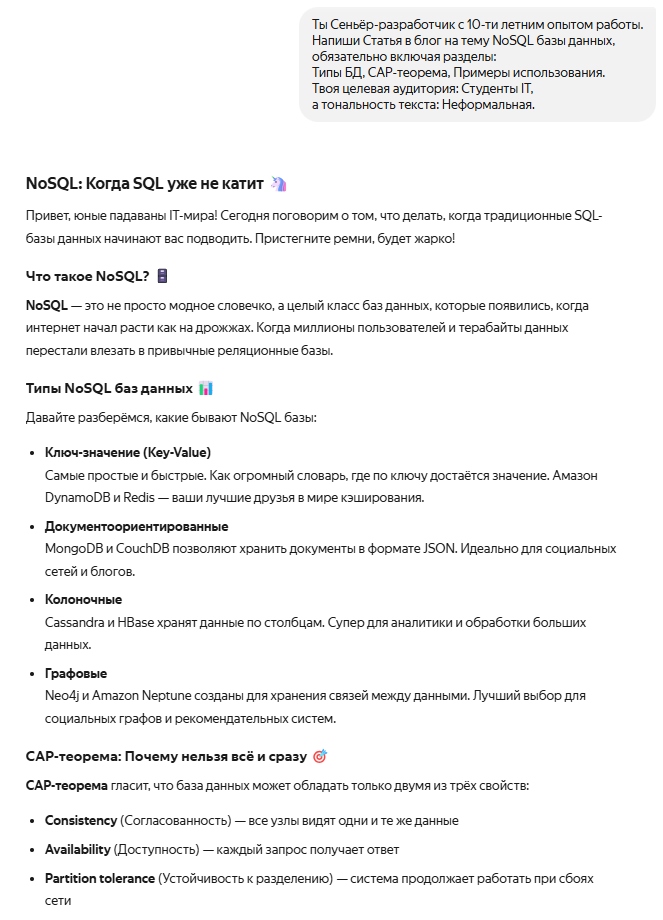
\includegraphics[width=16cm]{a1.png}
	\end{figure}
	\newpage
	\begin{figure}[H]
		\centering
		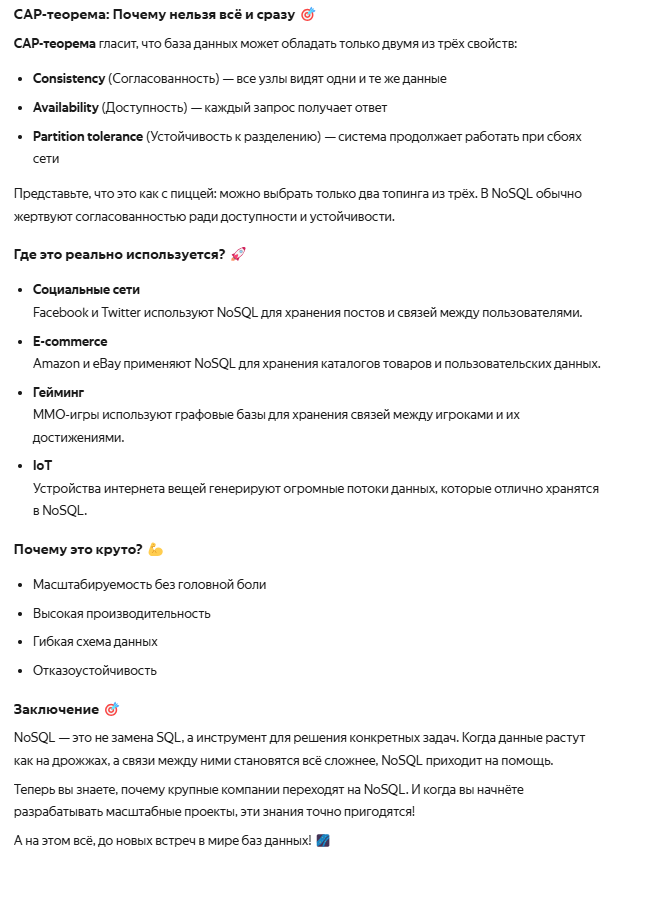
\includegraphics[width=16cm]{a2.png}
		\caption{Яндекс. Промпт v1: запрос и ответ}
	\end{figure}
	\newpage
	Модель от Яндекса отработала штатно, текст сгенерировала в обычной структере: введение, содержание, выводы. Все обязательные разделы присутствуют.

	\begin{figure}[H]
		\centering
		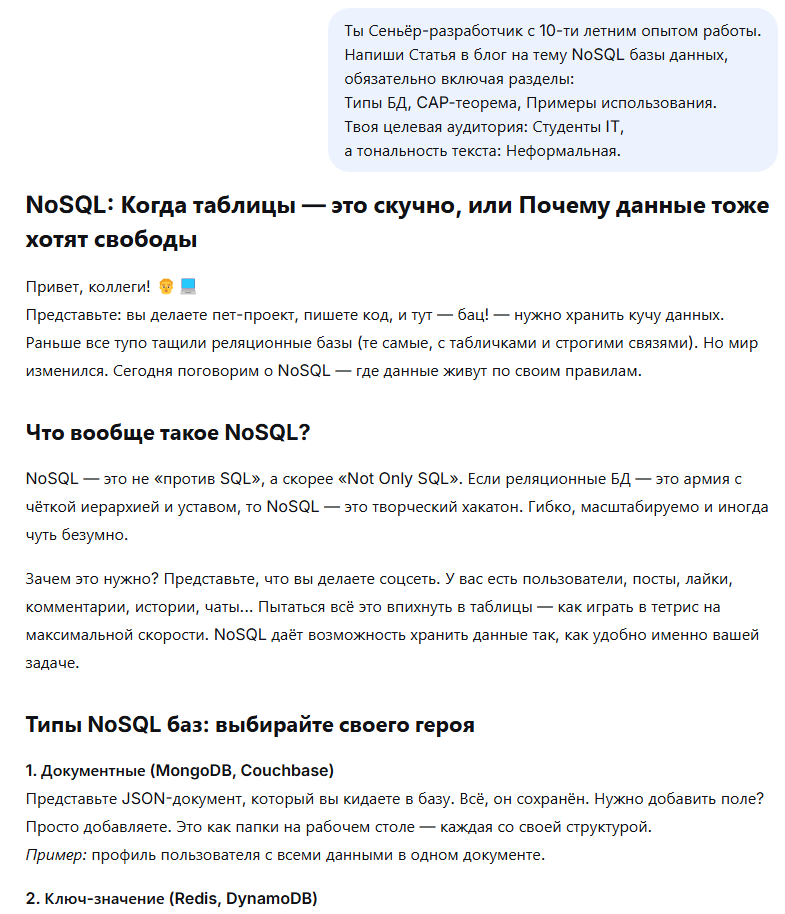
\includegraphics[width=16cm]{b1.png}
	\end{figure}
	\newpage
	\begin{figure}[H]
		\centering
		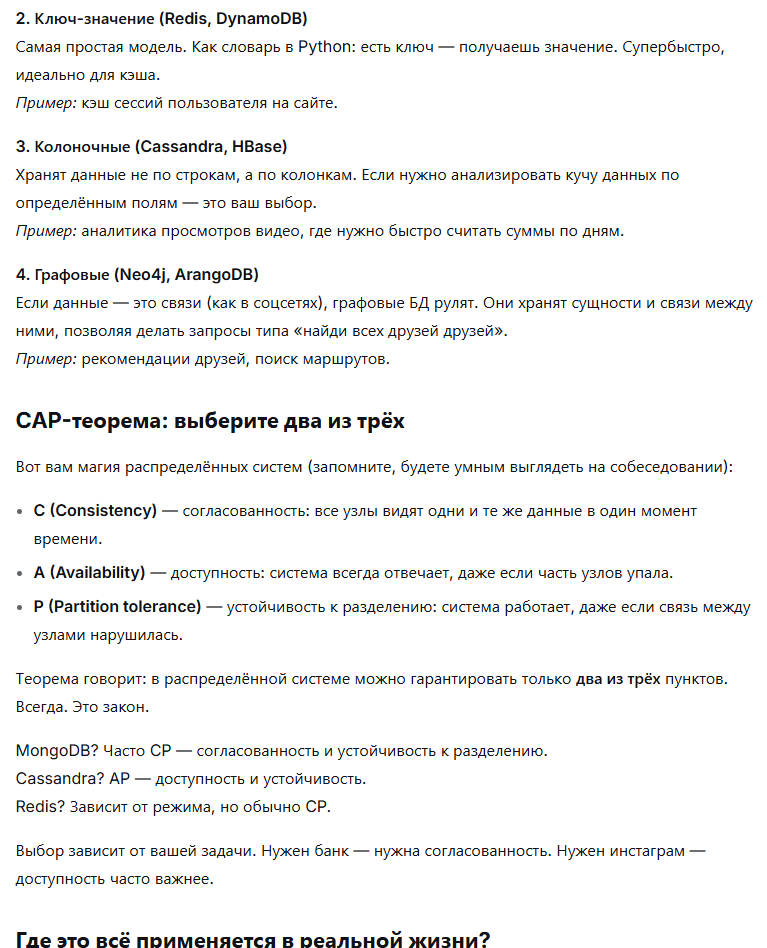
\includegraphics[width=16cm]{b2.png}
	\end{figure}
	\newpage
	\begin{figure}[H]
		\centering
		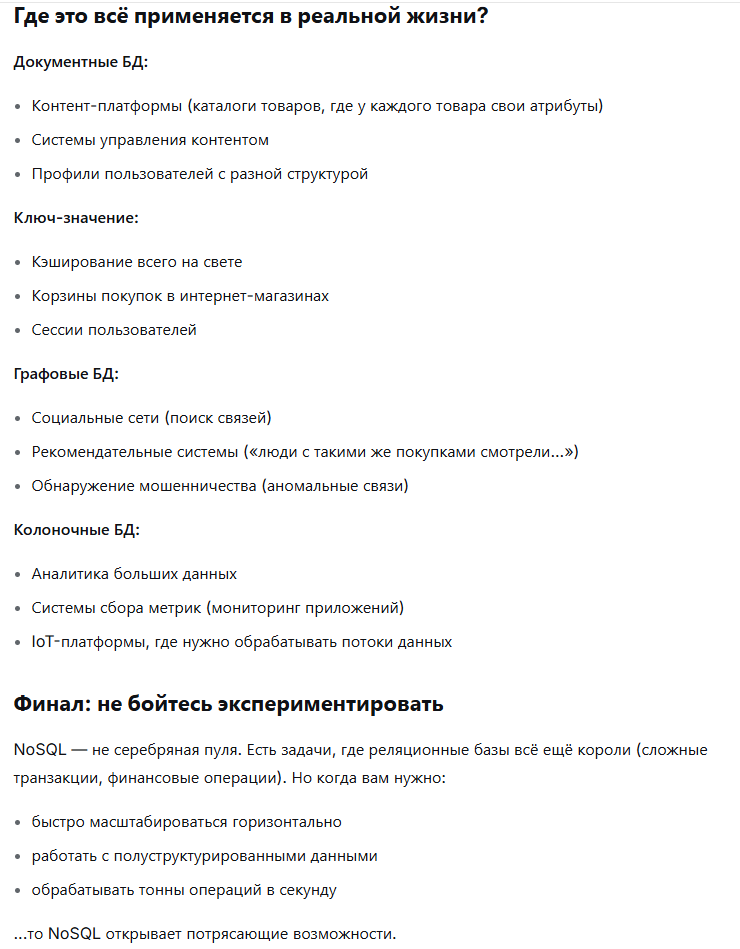
\includegraphics[width=16cm]{b3.png}
		\caption{DeepSeek. Промпт v1: запрос и ответ}
	\end{figure}
	\newpage
	Модель от DeepSeek тоже отработала штатно, соблюдая параметры, но текст вышел длиннее.
	
	\begin{table}[h!]
		\centering
		\begin{tabular}{|l|p{5cm}|p{5cm}|}
			\hline
			\textbf{Критерий} & \textbf{YandexGPT} & \textbf{DeepSeek} \\
			\hline
			Следование инструкции & 5 & 5 \\
			\hline
			Отсутствие галлюцинаций & 3 & 5 \\
			\hline
			Форматирование & 3 & 5 \\
			\hline
			Длинна текста & 5 & 4 \\
			\hline
			Источники информации & 3 & 5 \\
			\hline
			\textbf{Итог} & 3.8 & 4.8 \\
			\hline
		\end{tabular}
	\end{table}

	Модель от DeepSeek по многим критериям лучше: она ищет на разных источниках а не на первых как Яндекс, в тексте реже встречаются галлюцинации, но она любит раздувать текст. \\
	\newline
	Итоговый промпт:
	\begin{verbatim}
				Ты Сеньёр-разработчик с 10-ти летним опытом работы.
				Напиши {ТИП_ДОКУМЕНТА} на тему {ТЕМА},
				обязательно включая разделы: {РАЗДЕЛЫ}.
				Твоя целевая аудитория: {АУДИТОРИЯ},
				а тональность текста: {ТОНАЛЬНОСТЬ}.
	\end{verbatim}

\end{document}